

\section*{Supplementary Material}
\label{supp_results}

\maketitle

\subsection*{Application}

In the manuscript, we focused primarily on the outcome \textit{seizure freedom} as it has more unreported study outcomes and therefore provides a clearer visualization of our ORB adjustment method. For completeness, this section presents the corresponding plots for the second outcome \textit{50\% seizure reduction}.


\begin{figure}[ht!]
\centering
\caption{Outcome \textit{50\% seizure reduction}: comparison of naive and univariate ORB-adjusted estimates for selection on the log OR/ log RR and selection on the z-score over increasing selection.}
\label{fig:Univariate2}
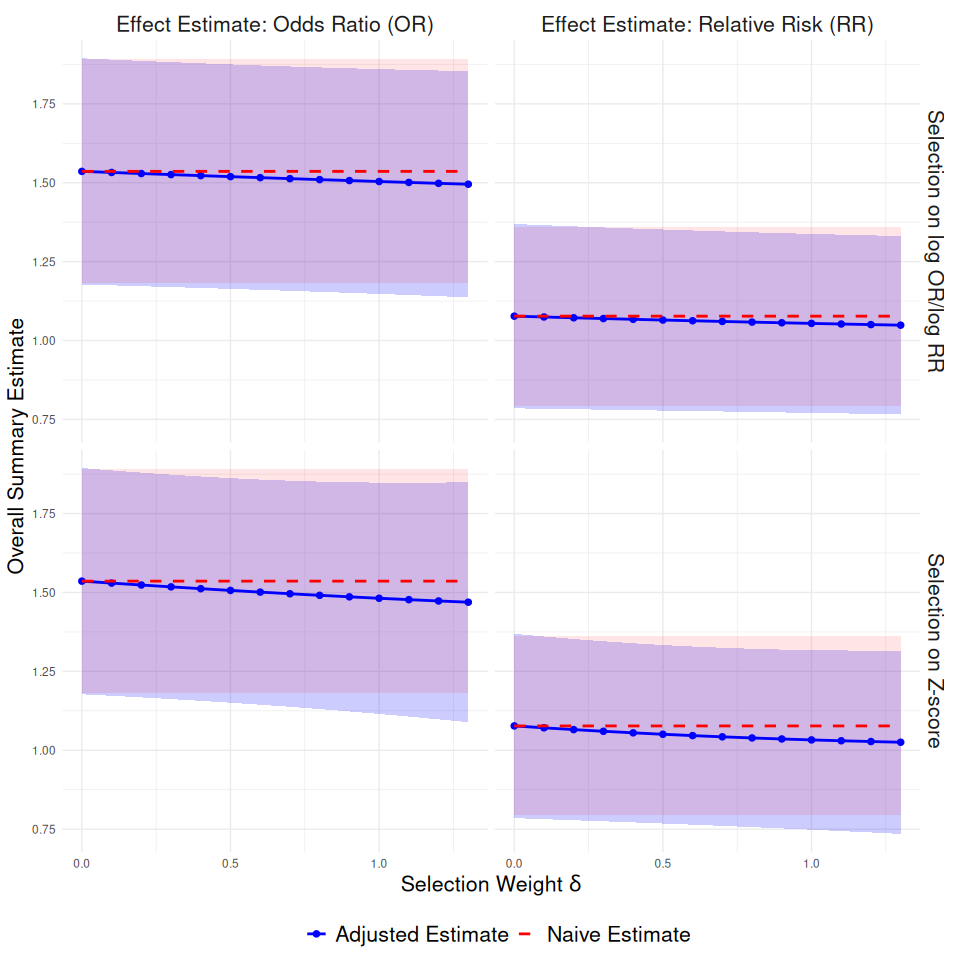
\includegraphics[width = 1\linewidth]{figures/App_Uni_REM_O1.png}
\end{figure}

As expected, the ORB-adjusted treatment effects and corresponding CIs are generally shifted toward the null compared to the naive MA estimates based only on the reported studies (Figure \ref{fig:Univariate2}). However, because only one study outcome is unreported for \textit{50\% seizure reduction}, the magnitude of the adjustment is substantially smaller than for \textit{seizure freedom}, where approximately half of the study outcomes are unreported. Consequently, the CIs of the naive and adjusted estimates are very similar. For both the OR and RR, selection on the z-score produces slightly stronger adjustment than selection on the effect estimate. This reflects the dependence of z-score selection on both the treatment effect and its standard error, giving greater influence to more precise studies as the selection weight increases. Similar to the findings for \textit{seizure freedom}, the OR estimates remain larger and have wider CIs  than the RR estimates. Overall, however, the differences between naive and adjusted estimates remain modest because the proportion of unreported study outcomes is small.

\begin{figure}[ht!]
\centering
\caption{Outcome \textit{50\% seizure reduction}: comparison of univariate and multivariate ORB-adjustment (for a correlation of $r = -0.3$) for selection on the log OR/ log RR and selection on the z-score over increasing selection.}
\label{fig:Uni_Multi_O1}
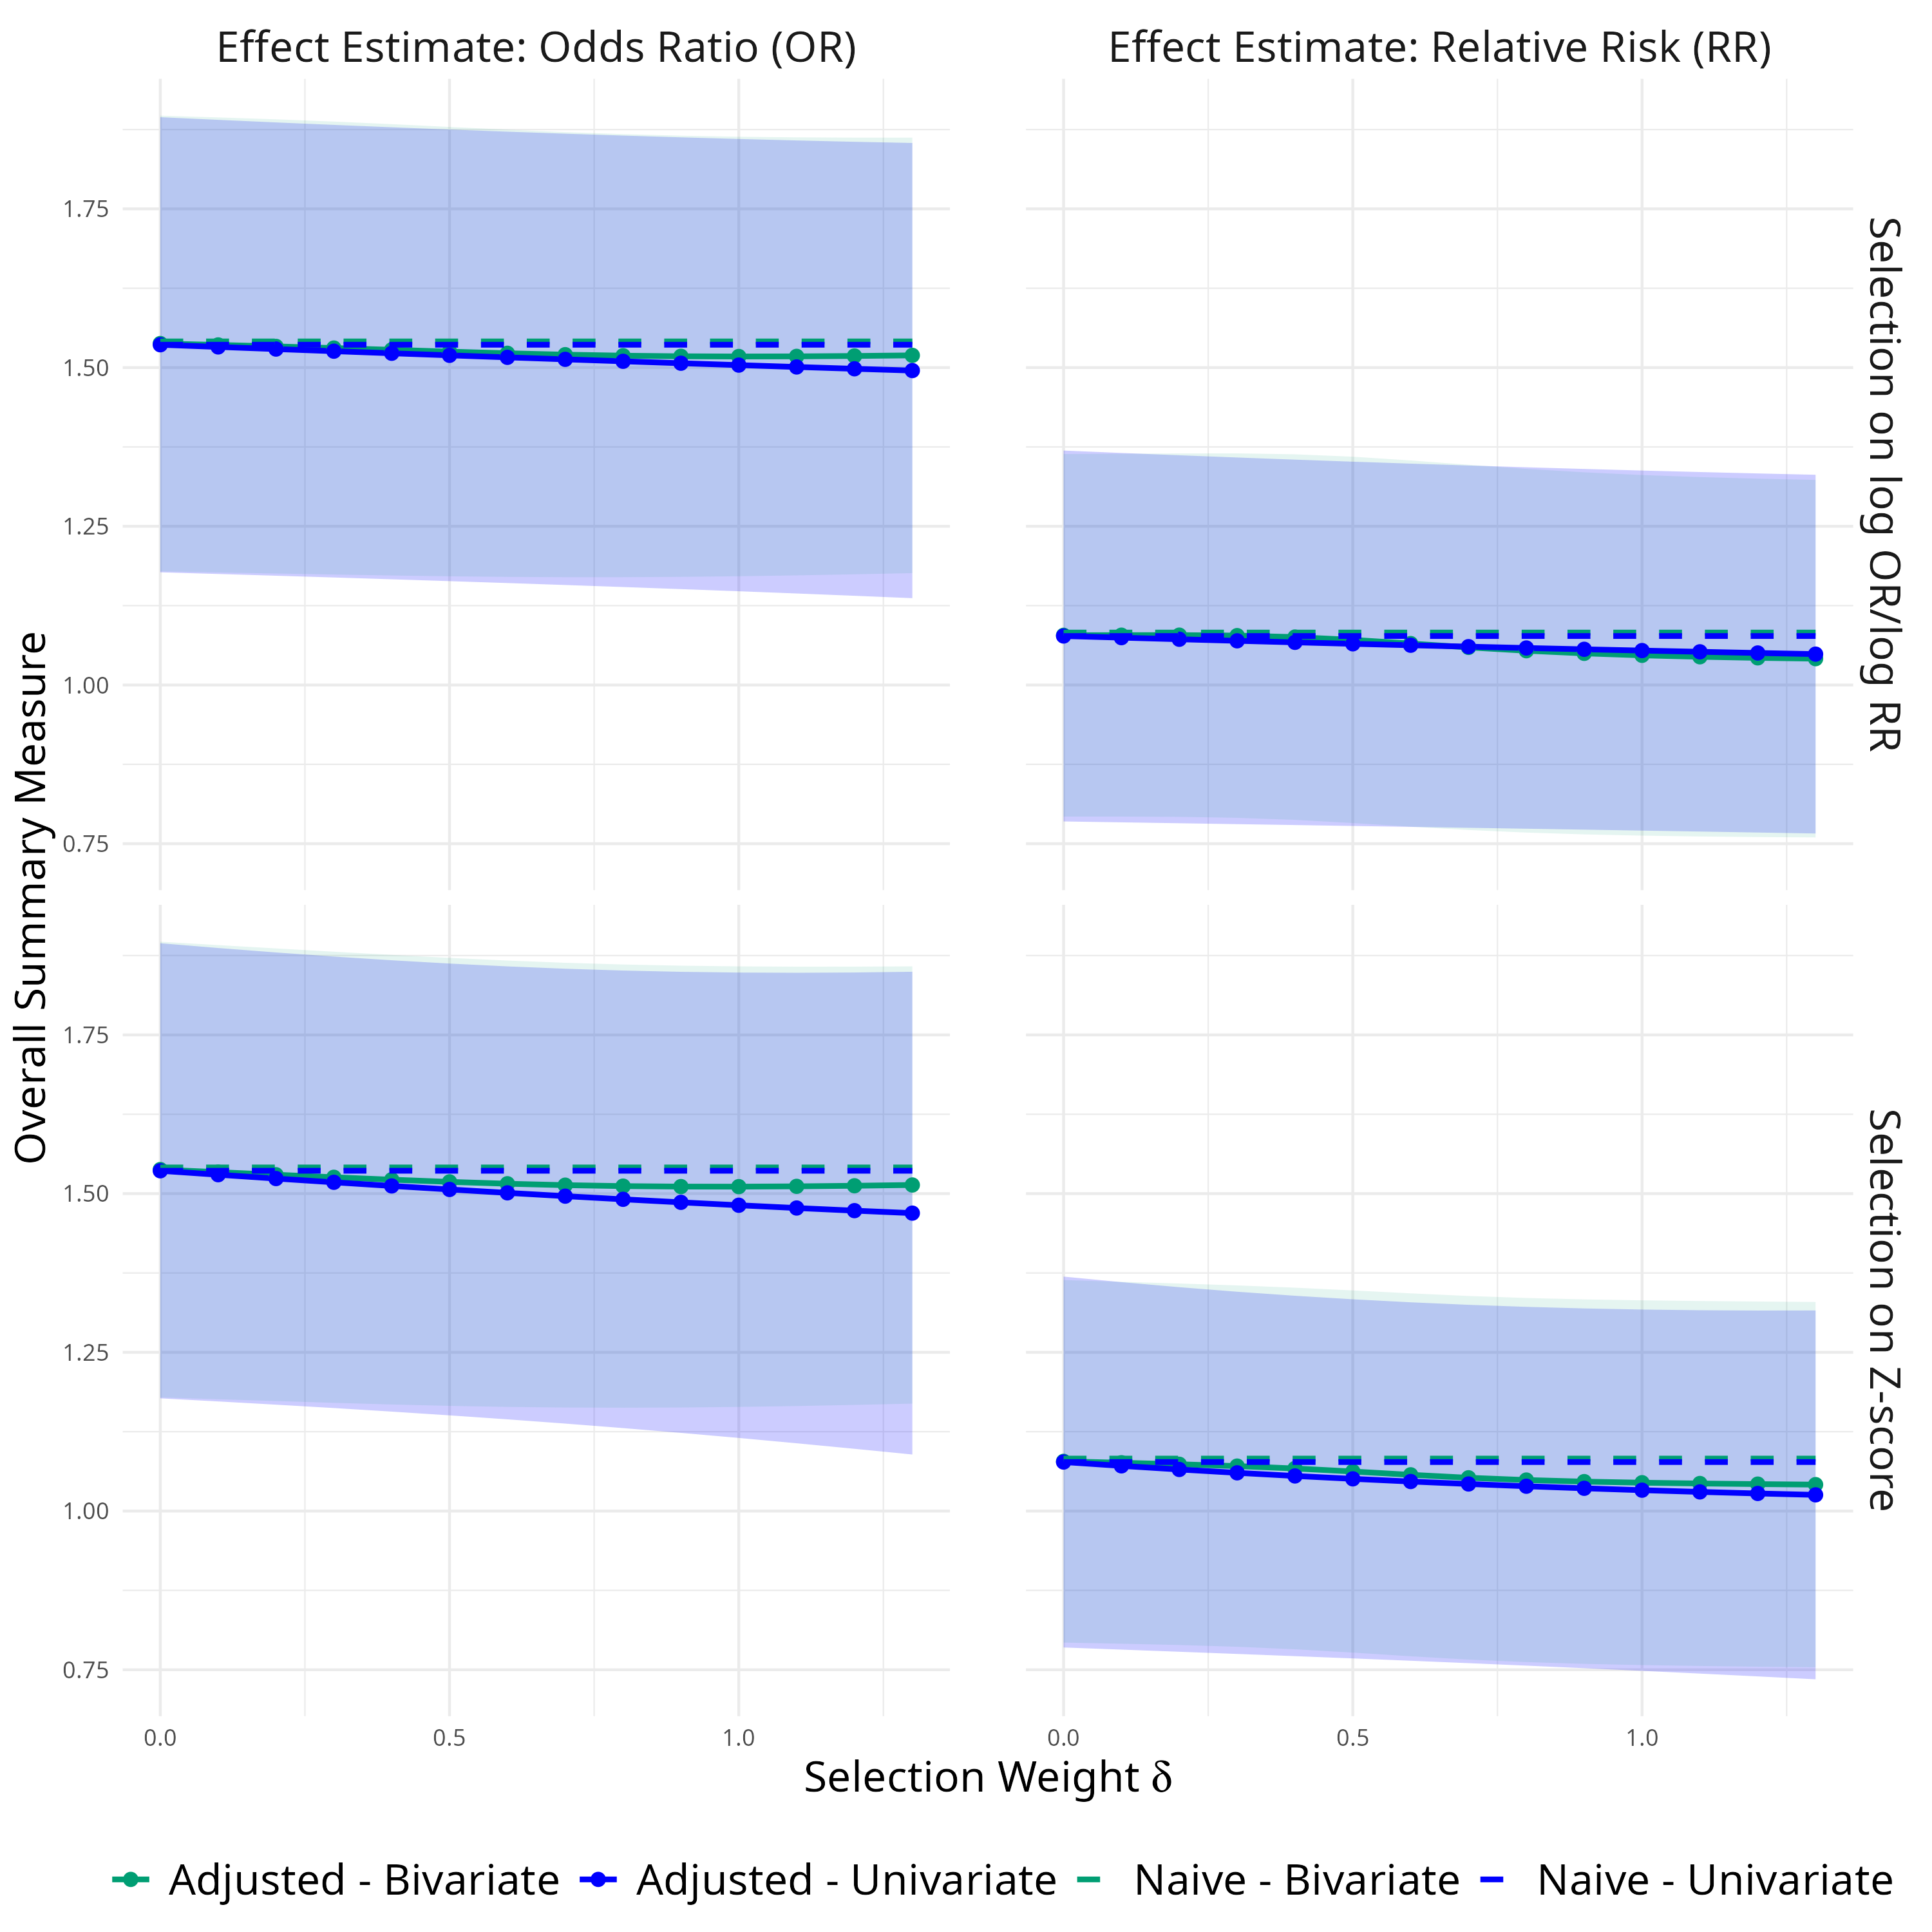
\includegraphics[width = 1\linewidth]{figures/Uni_Multi_Comp_12_REM_05_01.png}
\end{figure}

Next, we compared the univariate and multivariate ORB adjustment for the outcome \textit{50\% seizure reduction}, assuming a fixed within-study correlation of -0.3 (see Figure~\ref{fig:Uni_Multi_O1}). The dashed lines represent the naive MA estimates based only on the reported studies. These estimates differ between the univariate and multivariate approach because the multivariate model jointly incorporates both outcomes and their covariance structure. Across all scenarios, the adjusted estimates decrease with increasing selection, reflecting stronger assumed ORB. In contrast to the stronger differences observed for \textit{seizure freedom}, the univariate and multivariate adjustments for \textit{50\% seizure reduction} remain relatively similar, with largely overlapping CIs. For selection on the z-score, the univariate adjustment is slightly stronger than for selection on the effect estimate.

\begin{figure}[ht!]
\centering
\caption{Outcome \textit{50\% seizure reduction}: comparison of within-study correlations for multivariate ORB-adjustment for selection on the log OR/ log RR and selection on the z-score over increasing selection.}
\label{fig:Multivariate2}
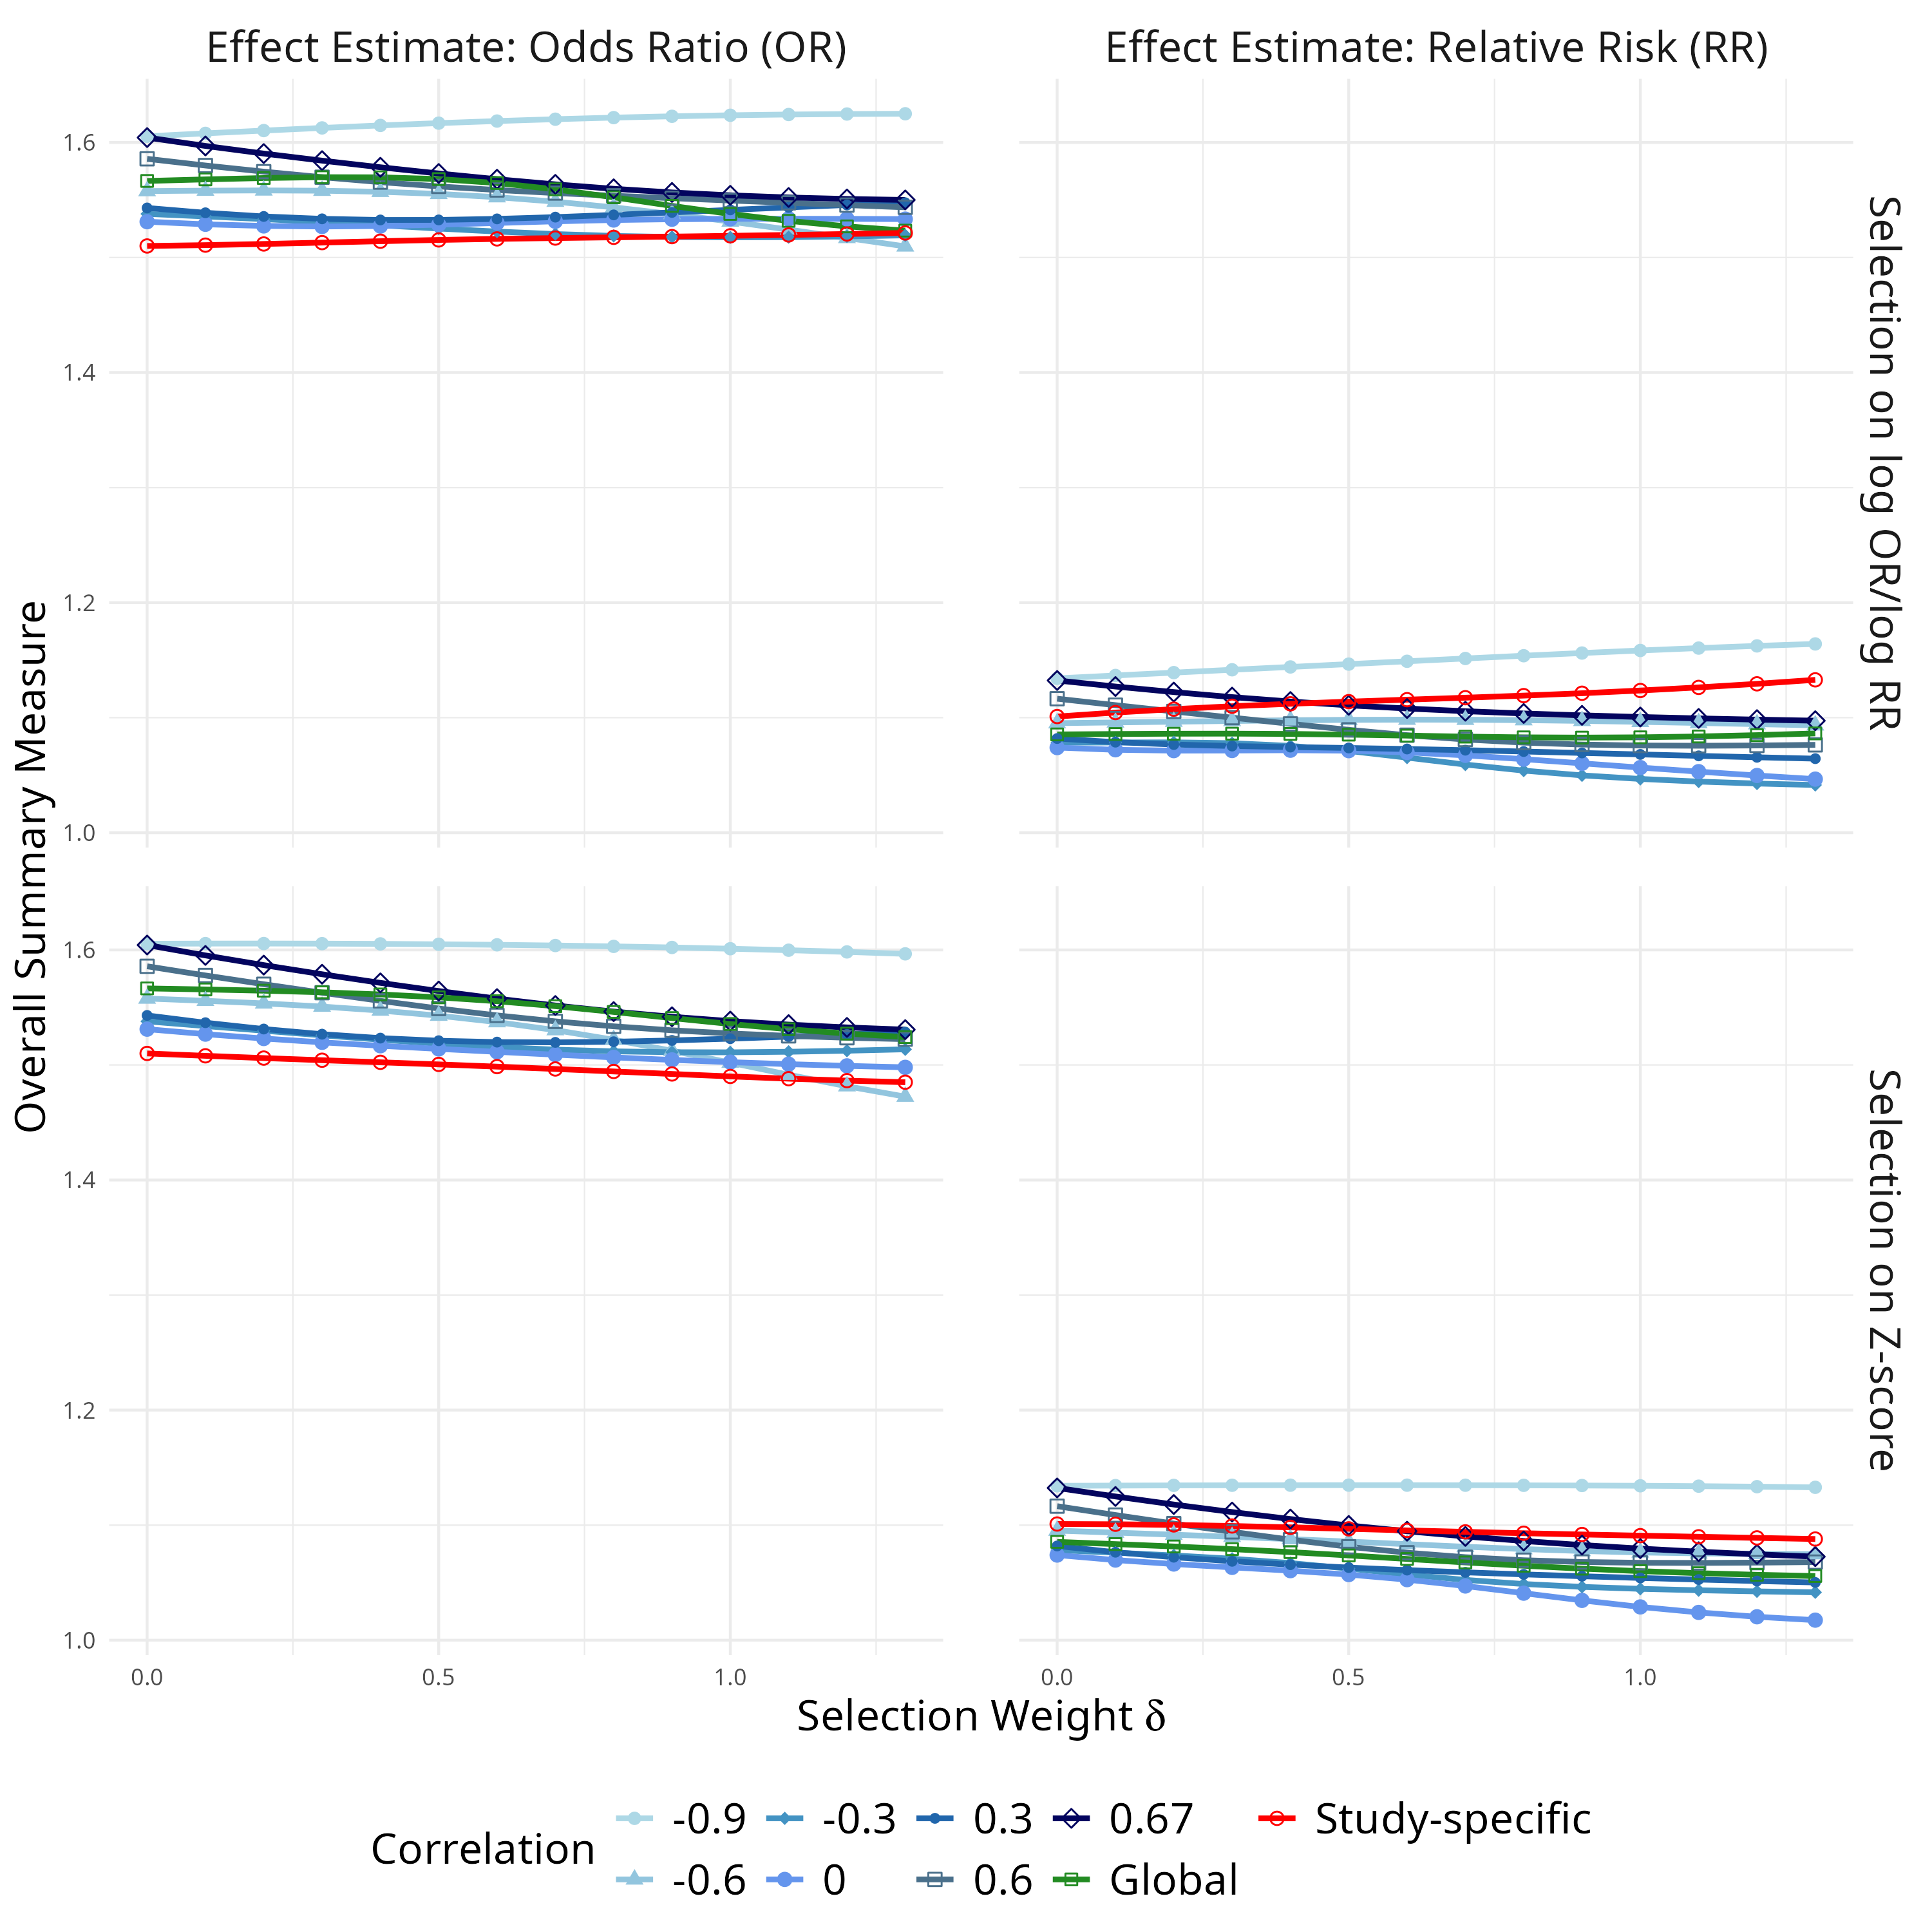
\includegraphics[width = 1\linewidth]{figures/App_Corr_12_mv_REM_O1.png}
\end{figure}

Figure \ref{fig:Multivariate2} compares the three approaches for incorporating within-study correlation for the outcome \textit{50\% seizure reduction}. In contrast to seizure freedom, only a single study outcome is unreported for this outcome. Consequently, the adjusted estimates are only weakly affected by the assumed within-study correlation, and the curves remain closely clustered across the full range of selection weights. Differences between correlation assumptions are already present at $\delta = 0$, reflecting the influence of the covariance structure on the imputed value under MAR. As the selection weight increases, the adjusted estimates change only modestly because the overall analysis is driven primarily by the reported outcomes. The study-specific correlation reflects the additional variability introduced by sampling a separate correlation for each study, although the overall differences remain small.

Overall, the results for \textit{50\% seizure reduction} demonstrate that the magnitude and stability of ORB adjustment depends strongly on the proportion of unreported study outcomes. When only a small proportion of outcomes is unreported, both univariate and multivariate adjustments remain relatively modest and robust to different modeling assumptions. In contrast, outcomes with a larger proportion of missing information are substantially more sensitive to assumptions regarding the selection mechanism and the within-study correlation structure. These findings highlight that multivariate ORB adjustment is most influential in settings with substantial selective non-reporting, where borrowing strength across correlated outcomes can alter the adjusted estimates and their uncertainty.

\subsection*{Simulation Study}
In the manuscript’s results section of the simulation study, we focus primarily on scenario where $\delta_{1,\text{sim}} = \delta_{1,\text{est}}$. This supplementary document presents additional results from the simulation study focusing on $\delta_{1,\text{sim}} \neq \delta_{1,\text{est}}$. 

The naive estimate exhibits the largest bias across nearly all scenarios (see Figure \ref{fig:App_Bias}). For both the univariate and bivariate ORB-adjusted estimates, bias generally increases as the assumed selection parameter $\delta_{1,\text{est}}$ deviates from the generating value $\delta_{1,\text{sim}}=0.8$, reflecting the impact of misspecifying the reporting mechanism. This effect is most pronounced under high heterogeneity ($I^2=90\%$). As in the main simulation results, bias is generally larger under selection on the z-score than under selection on the treatment effect. Variations in the number of studies have comparatively little influence on the magnitude of bias.

The MSE is also highest for the naive estimate and decreases over increasing sample size (see Figure \ref{fig:App_MSE}). Although both adjusted estimates exhibit increased MSE under stronger misspecification, their MSE remains substantially lower than that of the naive estimate. Differences between the univariate and bivariate ORB-adjusted estimates are generally small, indicating that both approaches remain reasonably robust to moderate misspecification of the selection parameter.


\begin{figure}[!ht]
\centering
\caption{Comparison of estimates for $\theta_1 = \theta_2 = 0.4$, $\rho_B = \rho_W = 0.4$, $p_i = 0.2$ and $\delta_{1,\text{sim}} = 0.8$. The bias is shown for varying meta-analysis study sizes, heterogeneity levels, selection type and an increasing selection weight in the estimation.}
\label{fig:App_Bias}
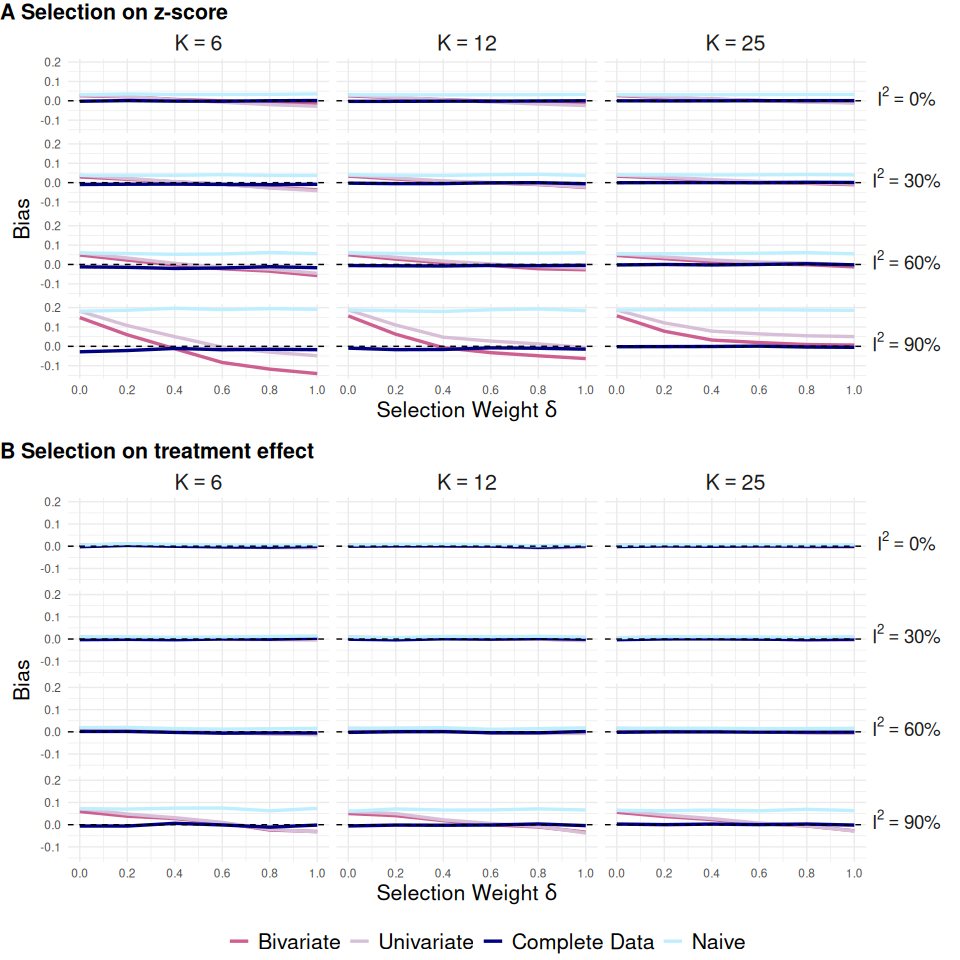
\includegraphics[width = 1\linewidth]{figures/Supp_SimStudy_Bias.png}
\end{figure}



\begin{figure}[!ht]
\centering
\caption{Comparison of estimates for $\theta_1 = \theta_2 = 0.4$, $\rho_B = \rho_W = 0.4$, $p_i = 0.2$ and $\delta_{1,\text{sim}} = 0.8$. The MSE is shown for varying meta-analysis study sizes, heterogeneity levels, selection type and an increasing selection weight in the estimation.}
\label{fig:App_MSE}
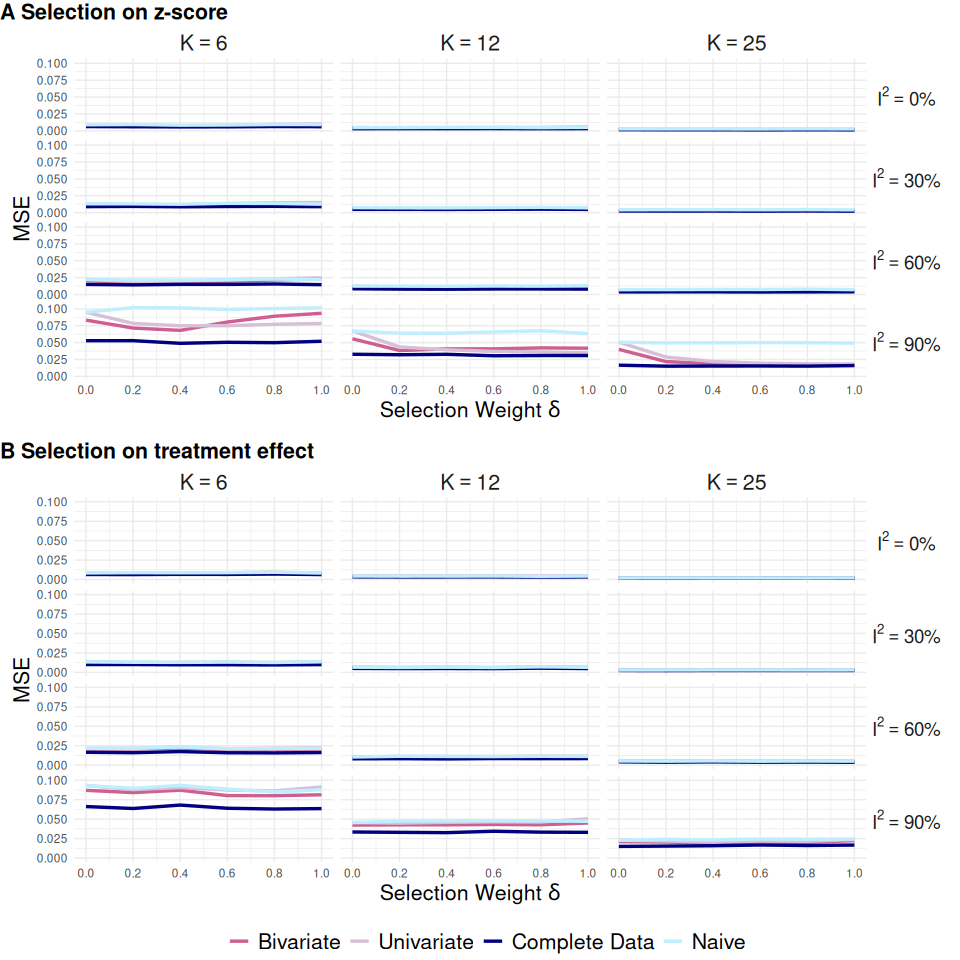
\includegraphics[width = 1\linewidth]{figures/Supp_SimStudy_MSE.png}
\end{figure}

CI widths decrease as the number of studies increases, reflecting improved estimation precision. For all scenarios except for high heterogeneity ($I^2 = 90\%$), the complete data estimate has the lowest CI width. For high heterogeneity ($I^2 = 90\%$) the univariate ORB-adjusted estimate has the lowest CI width, reflecting differences in the weighting and imputation procedures under severe selective reporting (see Figure \ref{fig:App_CI}).


\begin{figure}[!ht]
\centering
\caption{Comparison of estimates for $\theta_1 = \theta_2 = 0.4$, $\rho_B = \rho_W = 0.4$, $p_i = 0.2$ and $\delta_{1,\text{sim}} = 0.8$. The CI width is shown for varying meta-analysis study sizes, heterogeneity levels, selection type and an increasing selection weight in the estimation.}
\label{fig:App_CI}
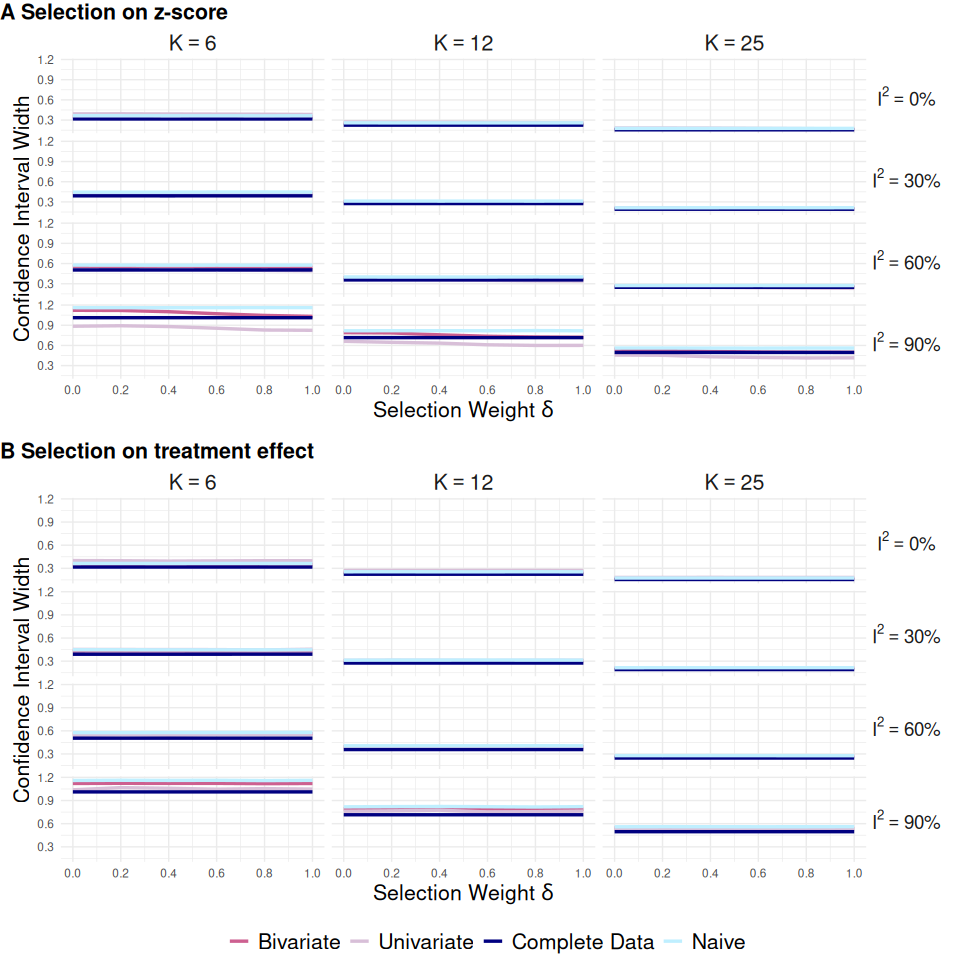
\includegraphics[width = 1\linewidth]{figures/Supp_SimStudy_CIWidth.png}
\end{figure}


As expected, the complete estimate maintains also for model misspecification nominal coverage at approximately 95\% across all simulated scenarios, serving as a reference baseline. The naive estimate shows acceptable nominal coverage when heterogeneity is low to moderate ($I^2 \le 60\%$). However, under strong heterogeneity ($I^2 = 90\%$), its performance degrades as the estimation selection weight increases. Particularly for large sample sizes ($K = 25$) under $z$-score selection coverage drops below 70\% (see Figure \ref{fig:App_Cov} A). The bivariate ORB-adjusted estimate demonstrates robust recovery of the nominal coverage probability across most scenarios. Under extreme heterogeneity ($I^2 = 90\%$), it exhibits a slight drop in coverage at lower estimation selection weights ($\delta < 0.4$) when the estimation model undercorrects for bias. However, it quickly converges toward nominal 95\% coverage as the estimated selection weight matches or approaches the generating parameter ($\delta_{\text{sim}} = 0.8$). The univariate adjusted method underperforms compared to the bivariate model, particularly under high heterogeneity ($I^2 \ge 60\%$) and when the estimated selection weight is low (see Figure \ref{fig:App_Cov}). This under-coverage may arise from a combination of residual variance underestimation and reduced borrowing of strength compared to the bivariate approach.


\begin{figure}[!ht]
\centering
\caption{Comparison of estimates for $\theta_1 = \theta_2 = 0.4$, $\rho_B = \rho_W = 0.4$, $p_i = 0.2$ and $\delta_{1,\text{sim}} = 0.8$. The coverage is shown for varying meta-analysis study sizes, heterogeneity levels, selection type and an increasing selection weight in the estimation.}
\label{fig:App_Cov}
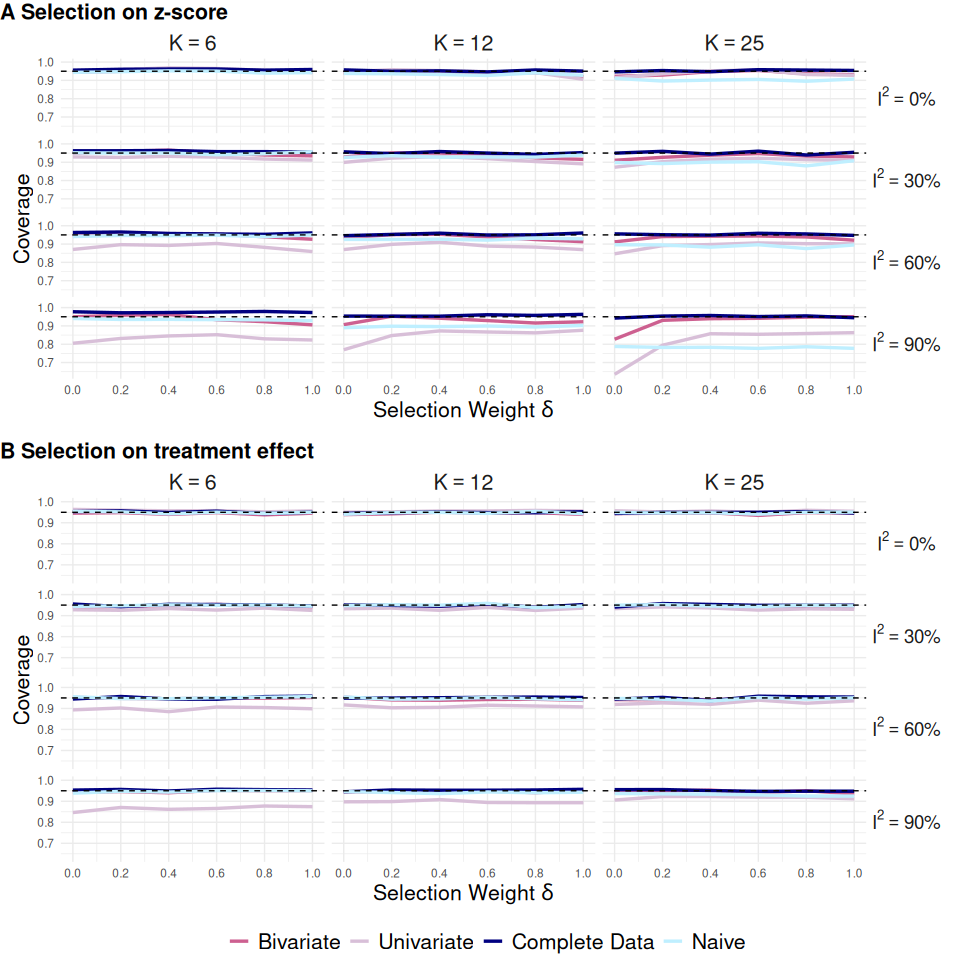
\includegraphics[width = 1\linewidth]{figures/Supp_SimStudy_Coverage.png}
\end{figure}

Overall, the additional analyses demonstrate that both ORB-adjusted methods have substantial advantages over the naive estimate even when the selection mechanism is misspecified. Although bias, MSE, and coverage deteriorate as the assumed selection parameter moves further away from the true generating value, the adjusted estimates generally continue to outperform the naive approach. In particular, the bivariate ORB-adjusted method remains comparatively robust across the considered misspecification scenarios, maintaining lower bias and MSE together with coverage closer to the nominal level. 